%==================================================
% This is for generating a standalone of the evaluation document
%==================================================
\documentclass[a4paper, 11pt]{report}
\usepackage[T1]{fontenc}
\usepackage[utf8]{inputenc}
\usepackage[english]{babel}
\usepackage{graphicx} % support graphics
\usepackage{hyperref} % links in the document
\usepackage{float} % position of figures
\usepackage{paralist} % inline lists
\usepackage{verbatim} % multiline comments
\usepackage[table]{xcolor} % table row coloring
\usepackage{booktabs} % Professional tables
\usepackage{tabularx} % Simple column stretching
\usepackage{multirow} % Row spanning
\usepackage{wrapfig} % Wrap text around figures
\usepackage{array}
\usepackage{listings}
\usepackage{color}
\usepackage{textcomp}
\usepackage[style=treenoname,subentrycounter,numberedsection, 
        section=chapter, acronym]{glossaries}


\definecolor{listinggray}{gray}{0.9}
\definecolor{lbcolor}{rgb}{0.9,0.9,0.9}

\lstset{
    backgroundcolor=\color{lbcolor},
    tabsize=4,
    rulecolor=,
    language=C,
    basicstyle=\footnotesize,
    upquote=true,
    aboveskip={1.5\baselineskip},
    columns=fixed,
    showstringspaces=false,
    extendedchars=true,
    breaklines=true,
    prebreak = \raisebox{0ex}[0ex][0ex]{\ensuremath{\hookleftarrow}},
    frame=single,
    showtabs=false,
    showspaces=false,
    showstringspaces=false,
    identifierstyle=\ttfamily,
    keywordstyle=\color[rgb]{0,0,1},
    commentstyle=\color[rgb]{0.133,0.545,0.133},
    stringstyle=\color[rgb]{0.627,0.126,0.941},
}

% Configure links in pdfs
\hypersetup{
    bookmarksopen=false, % Hide bookmarks menu
    colorlinks=true, % Don't wrap links in colored boxes
}

\title{Evaluation}
\author{Kpro group 9}
\date{\today}

\begin{document}
%\maketitle
%\tableofcontents
\makeglossaries
\newglossaryentry{wireshark}{name={Wireshark},
description={Program used to analyze packet data sent between network nodes}}

\newglossaryentry{python}{name={Python},
description={A programming language}}

\newglossaryentry{mac}{name={Mac},
description={A brand of personal computers}}

\newglossaryentry{linux}{name={Linux},
description={An operating system}}

\newglossaryentry{c}{name={C},
description={A programming language}}

\newglossaryentry{clang}{name={clang},
description={A compiler front-end for different \Gls{c} programming languages}}

\newglossaryentry{gcc}{name={gcc},
description={define this}}

\newglossaryentry{c++}{name={C++},
description={A programming language}}

\newglossaryentry{java}{name={Java},
description={A programming language}}

\newglossaryentry{lua}{name={Lua},
description={A programming language, often used for making \glspl{script}}}

\newglossaryentry{script}{name={script},
description = {A list of commands that are executed by a certain program, usually as an extension of the original functionality},
plural=scripts} 

\newglossaryentry{int}{name={int},
description={See \gls{integer}}}

\newglossaryentry{double}{name={double},
description={DEFINE}}

\newglossaryentry{integer}{name={integer},
description={define this},
plural=integers}

\newglossaryentry{char}{name={char},
description={define this},
plural=chars}

\newglossaryentry{float}{name={float},
description={define this},
plural=floats}

\newglossaryentry{pycparser}{name={pycparser},
description={A \Gls{c} \gls{parser} written in \Gls{python}}}

\newglossaryentry{ply}{name={ply},
description = {A \Gls{python} \gls{library} for creating \glspl{lexer} and \glspl{parser}}}

\newglossaryentry{parser}{name={parser},
description = {A program that receives input, checks it for correct syntax and builds a data structure representing the input},
plural=parsers}

\newglossaryentry{lexer}{name={lexer},
description = {A lexer is a program that converts a sequence of characters into a sequence of tokens},
plural=lexers}

\newglossaryentry{token}{name={token},
description = {A string of characters, categorized as a symbol according to a set of given rules},
plural=tokens}

\newglossaryentry{dissector}{name={dissector},
description = {Code that decodes \gls{packet} data and makes it readable by humans},
plural=dissectors}

\newglossaryentry{packet}{name={packet},
description = {Small block of data transmitted over a network},
plural=packets}

\newglossaryentry{utility}{name={utility},
description = {A small program that supports larger applications by doing certain tasks},
plural=utilities}

\newglossaryentry{library}{name={library},
description = {A collection of pre-written code for aiding programmers in the development process},
plural=libraries}

\newglossaryentry{ipc}{name={inter-process communication},
description = {The exchange of data that happens between \glspl{process}}}

\newglossaryentry{process}{name={process},
description = {A program running on a computer},
plural=processes}

\newglossaryentry{struct}{name={struct},
description = {Short for structure, it is a type that groups several \glspl{member} into a single \gls{object}},
plural=structs}

\newglossaryentry{member}{name={member},
description = {define this},
plural=members}

\newglossaryentry{binary}{name={binary},
description = {Two base arithmetic using the digits 0 and 1}}

\newglossaryentry{binary file}{name={binary file},
description = {A computer-readable file stored in \gls{binary} format}}

\newglossaryentry{nested struct}{name={nested struct},
description = {A \gls{struct} within another \gls{struct}},
plural={nested structs}}

\newglossaryentry{sparc}{name={SPARC},
description={A microprocessor architecture based on reduced instruction set computing}}

\newglossaryentry{version control system}{name={version control system},
description = {A system that ensures consistency of files when several people are collaborating on them},
plural={version control systems}}

\newglossaryentry{scrum}{name={Scrum},
description={A \gls{software development methodology}}}

\newglossaryentry{software development methodology}{name={software development methodology},
description={A framework used to structure, plan and control a development process},
plural={software development methodologies}}

\newglossaryentry{branch}{name={branch},
description={define this},
plural=branches}

\newglossaryentry{distributed repository model}{name={distributed repository model},
description={A distributed approach to a \gls{version control system}},
plural={distributed repository models}}

\newglossaryentry{markup language}{name={markup language},
description={A language for specifying the processing, definition and presentation of text}}

\newglossaryentry{capture file}{name={capture file},
description={A file containing the data that is captured from network or IPC traffic},
plural={capture files}}

\newglossaryentry{ascii}{name={ASCII},
description={A character encoding scheme}}

\newglossaryentry{character encoding scheme}{name={character encoding scheme},
description={A system that maps characters to something else, write more }}

\newglossaryentry{hexadecimal}{name={hexadecimal},
description={A number system where sixteen is the base}}

\newglossaryentry{hex dump}{name={hex dump},
description={A \gls{hexadecimal} view of computer data},
plural={hex dumps}}

\newglossaryentry{pcap-file}{name={pcap-file},
description={See \gls{capture file}},
plural={pcap-files}}

\newglossaryentry{protocol}{name={protocol},
description = {A system of rules for exchanging messages between machines},
plural=protocols}

\newglossaryentry{link-layer}{name={link-layer},
description = {The \gls{protocol} layer that is responsible for transferring data between two nodes}}

\newglossaryentry{repository}{name={repository},
description = {A central storage area where data is kept and maintained},
plural=repositories}

\newglossaryentry{Sun RPC}{name={Sun RPC},
description={The Unix equivalent of Remote Procedure Call}}

\newglossaryentry{corba}{name={CORBA},
description={This is an acronym}}

\newglossaryentry{asn1}{name={ASN.1},
description={This is an acronym}}

\newglossaryentry{makefile}{name={makefile},
description={A file that helps the make utility in the creation of executables from source code},
plural=makefiles}

\newglossaryentry{post-dissector}{name={post-dissector},
description = {define this},
plural=post-dissectors}

\newglossaryentry{boolean}{name={boolean},
description={A data type that represents logical truth, it has the value True or False},
plural=booleans}

\newglossaryentry{string}{name={string},
description={define this},
plural=strings}

\newglossaryentry{garbage collection}{name={garbage collection},
description={define this}}

\newglossaryentry{closure}{name={closure},
description={define this},
plural=closures}

\newglossaryentry{object}{name={object},
description = {define this},
plural=objects}

\newglossaryentry{C99}{name={C99},
description={define this}}

\newglossaryentry{GCC-XML}{name={GCC-XML},
description={define this}}

\newglossaryentry{xml}{name={xml},
description={A \gls{markup language}}}

\newglossaryentry{Objective-C++}{name={Objective-C++},
description={A programming language}}

\newglossaryentry{Objective-C}{name={Objective-C},
description={A programming language}}

\newglossaryentry{AST}{name={abstract syntax tree},
description={A tree represention of a compiled program}}

\newglossaryentry{data serialization}{name={data serialization},
description={define this}}

\newglossaryentry{perl}{name={perl},
description={A programming language}}

\newglossaryentry{php}{name={php},
description={A scripting language}}

\newglossaryentry{Ruby}{name={Ruby},
description={A programming language}}

\newglossaryentry{Javascript}{name={Javascript},
description={A scripting language}}

\newglossaryentry{Eclipse}{name={Eclipse},
description={An application aiding computer programmers in software development}}

\newglossaryentry{header}{name={header},
description={define this},
plural=headers}

\newglossaryentry{enumerated named value}{name={enumerated named value},
description={define this},
plural={enumerated named values}}

\newglossaryentry{union}{name={union},
description={define this},
plural=unions}

\newglossaryentry{array}{name={array},
description={A data type that can hold a collection of elements},
plural=arrays}

\newglossaryentry{preprocessor}{name={preprocessor},
description={Define this},
plural=preprocessors}

\newglossaryentry{include}{name={\#include},
description={A \Gls{c} directive that includes other \gls{header} files to the current file}}

\newglossaryentry{if}{name={\#if},
description={A \Gls{c} directive that executes a statement if a given expression holds true }}

\newglossaryentry{ifdef}{name={\#ifdef},
description={A \Gls{c} directive that checks if a given token has been defined}}

\newglossaryentry{define}{name={\#define},
description={A \Gls{c} directive that can be used to define a constant or create a macro}}

\newglossaryentry{trailers}{name={trailers},
description={define this}}

\newglossaryentry{bit string}{name={bit string},
description={define this}
plural={bit strings}}

\newglossaryentry{endian}{name={endian},
description={See \gls{endianness}},
plural=endians}

\newglossaryentry{endianness}{name={endianness},
description={Refers to the ordering of bytes in a word. A big-endian machine stores the most significant byte first, and a little-endian the least significant.}}

\newglossaryentry{batch mode}{name={batch mode},
description={define this}}

\newglossaryentry{batch processing}{name={batch processing},
description={See \gls{batch mode}}}

\newglossaryentry{x86}{name={x86},
description={The instruction set architecture used by Intel processors}}

\newglossaryentry{Windows}{name={Windows},
description={An operating system by Microsoft}}

\newglossaryentry{Solaris}{name={Solaris},
description={An operating system by Sun Microsystems}}

\newglossaryentry{x86-64}{name={x86-64},
description={An extension of the \gls{x86} instruction set that is compatible with 64-bit processors}}

\newglossaryentry{Field}{name={Field},
description={define this}}

\newglossaryentry{argparse}{name={argparse},
description={define this}}

\newglossaryentry{enum}{name={enum},
description={See /gls{enumerated named value}},
plural=enums}

\newglossaryentry{wildcard}{name={wildcard},
description={define this}}

\newglossaryentry{x-86}{name={x-86},
description={define this}}



\newacronym{ntnu}{NTNU}{Norwegian University of Technology and Science}
%========================================
\chapter{Architectural Description}
%========================================
This chapter introduces the final architectural documents for the project. The team followed the definition of software architecture defined by Len Bass, Paul Clements and Rick Kazman: ``The software architecture of a program or computing
system is the structure of structures of the system, which comprise software elements, the externally visible properties of those elements, and the relationships between them.''~\cite[p.3]{Bass2003}

The purpose of this document is to describe our architecture in a structured way so that it can be used, not only by the team, but also as an aid for other stakeholders who are trying to understand the system.

%-------------------------------------
\section{Architectural Drivers}
%-------------------------------------
This section is dedicated to the discussion of the architectural drivers that were discovered during the project.
The team chose Modifiability and Testability as quality attributes, but it later on became apparent that some care should also be taken considering Performance.

The reason for choosing Modifiability was that the development team would be unable to update or maintain the \gls{utility} after completing this project. The code would also be distributed under a GPL which allows other developers to continue working on the utility and use it for their own applications in the future. It was therefore important that the code would be easy to understand, well documented and easy to modify. Not only will this promote the further development of the utility, but it would also make it easier for the customer to use and modify for their own purposes.

Testability would also be an important quality attribute as the \gls{utility} was to be used by the customer for debugging purposes. It was therefore be very important that the utility it self contained as few bugs as possible so that the customer could be sure that the output given by the utility would be able to help them in analyzing and debugging. The developers of this project were also unable to test any given \glspl{dissector} in a real environment, which made it even more necessary for the developers to do extensive testing of the utility's functionality. This was to ensure that the final product works properly even without the developers having had taken a good look on the data the utility will have to process after going public.

Performance became somewhat of an issue for the utility during the project as it became apparent that the customer would have to run the utility on several thousand header files at once. It would therefore be important for the utility to be able to run through all of the customer's header files in a reasonable amount of time, which in this case would be that the utility should be able to run through several thousand header files over one night of being run in batch mode.

\subsection{Testability Tactics}
%------------------------------------
The goal of using testability tactics was making it easier to test the system after finishing any given sprint, as well as generally raising the quality of the tests and the amount of coverage the tests give the system.

\subsubsection{Specialize Access Routes/Interfaces}
Using a specialized testing interface makes it possible to specify values for a component independently from its normal execution. This will in turn make it possible to test parts of an unfinished module as well as making it easier to get a clear overview over what data is flowing through individual parts of the system. This is important for this project as the \gls{utility} must be able to run in a different environment than what the developers have access to. The testers must therefore be able to create input for each individual component of the system in order to ensure that it will work correctly with all kinds of input.

We incorporated the use of this tactic by using the Attest testing framework when creating unit tests. By using attest we were able to create instances of and test parts and modules of the system independently with the exact input we wanted without having to run the entire utility. 

\subsubsection{Code Coverage}
By using a framework to see which parts and how much of the code is actually being run during the unit tests, it becomes easier to improve the quality of the unit tests. It could also be used as a checklist to see if the ones creating the unit tests have implemented some functionality that is currently not being tested.

We incorporated the use of this tactic by using the Coverage tool for python. By using coverage we were able to measure the code coverage of the unit tests by having Coverage create a html table which showed which parts and percentage of the system actually underwent testing.

\subsection{Modifiability Tactics}
%-------------------------------------------
The goal of using modifiability tactics were to make it easer to extend and modify the software during development as well as after completing the product.

\subsubsection{Anticipate Expected Changes}
By trying to anticipate expected changes it is possible to make it easier for modules to be extended with new functionality later. It also makes it easier for the developers to anticipate the different ranges of input the modules are able to process. This was important for this project as it was being developed incrementally, with new functionality and code added every sprint.

This was handled in this project by first identifying all of the functionality that the utility would need in order to be considered a finished product. Then we had some discussions about what should be included in each following sprint, where it was also discussed in minor detail how the work items were to be implemented. This made it easier for the developers to figure out which changes might have to be done further down the line so that they could prepare their code beforehand.

\subsubsection{Generalizing Modules}
Generalizing the modules of a system makes it possible to reuse older modules when doing modifications to the system. The more general a module, the more likely it is that a needed change to the system can be implemented by just adjusting the input to the system, rather than having to modify existing or creating new modules.

This was implemented mostly by using inheritance where we reused a lot of the functionality in a class when making new classes that needed similar functionality.

\subsubsection{Restrict Communication Paths}
By restricting the number of modules that are able to collect data from a specific module, the less dependent the entire system becomes of that specific module. This makes it easier to swap out existing modules with new ones without having to make many widespread changes to the entire system. This is important for this project as the source code could change drastically after discovering new requirements in later sprints. By having a loose coupling we will minimize the amount of code that has to be rewritten after every sprint.

We followed this tactic by using code inspection. If we discovered during a sprint that the coupling between the modules were becoming too tight, it was decided to refactor some of the code early on in order to save time by not having to do any major refactoring later on.

\subsubsection{Using Configuration Files}
By using configuration files, it is possible to change the behaviour of the system without having to do any changes to its code. It is very important that this system uses configuration files as this was a requirement from the customer, as well as making it a lot more flexible for the end user.

In order to implement this in the project it was decided that we would use the YAML format for writing and parsing configuration files. These configuration files would then make it possible for the users of the utility to make several alterations to how data should be displayed in Wireshark as well as having their own custom LUA code that would get run inside of the generated dissectors.

\subsection{Business Requirements}
%---------------------------------
The following business requirements encompass the most important needs of the customer.
\begin{itemize}
\item The \gls{utility} must be delivered on time as it is not possible for the
developers to continue the development after the deadline
\item The utility should be able to create dissectors for the C-structs in
header files used by Thales
\item The utility should be able to create dissectors that run on all of the
platforms used by Thales and their customers
\item Developers at Thales should be able to use Glswireshark with the generated
dissectors to display the values in C-structs passed through the
system.
\end{itemize}

\subsection{Design Goals}
%------------------------
To help guide the design and the implementation we tried to follow these goals and guidelines:
\begin{itemize}
	\item Smart data structures and dumb code works better than the other way around~\cite{Raymond1999}!
	\item Clear and clean separation of the front-end and the back-end so in the future other parsers can be used to generate \glspl{dissector}.
	\item Try to be pythonic, follow  PEP8 \footnote{Style Guide for Python Code: \url{http://www.python.org/dev/peps/pep-0008/}} and PEP20\footnote{The Zen of Python \url{http://www.python.org/dev/peps/pep-0020/}}.
	\item Now is better than never. Don't be afraid to write stupid or ugly code, we can always fix it later.
	\item The first version is never perfect, so don't wait until its perfect before you commit. Commit often!
\end{itemize}

%------------------------------
\section{Architectural Patterns}
%------------------------------
This section presents the different architectural patterns used in the \gls{utility}

\subsection{Pipe and Filter}
%---------------------------
The pipe and filter architectural pattern consists of a stream of data that in turn is processed sequentially by several filters. This is done in such a fashion that the output of one filter becomes the input of the other. It is a very flexible, yet robust way of processing data, with support for adding more filters if needed for future applications and processes. As the \gls{utility} will only work on one piece of data that gradually changes, and is then converted into \Gls{lua}-code at the end, this seemed like a good and structured way of processing data early on, while still being able to add new functionality further down the line.

\begin{figure}[htb]
	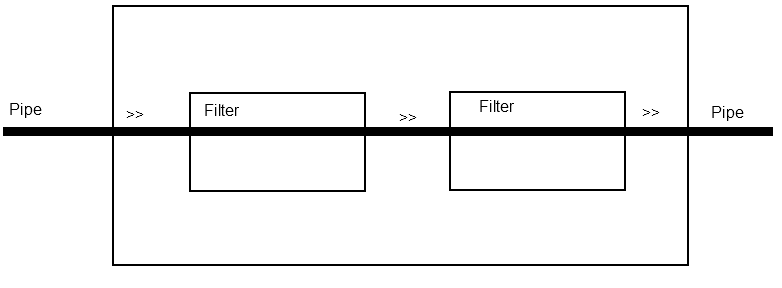
\includegraphics[width=\textwidth]{./planning/img/PipeAndFilter}
	\caption{Pipe and Filter Pattern\label{fig:pipefilter}}
\end{figure}

\subsection{Layered Architectural Pattern}
%-------------------------------------------------
\label{sec:Layered}
The layered architectural pattern is a pattern that involves grouping several different classes that all share the same dependencies. This grouping of classes is called a layer, and the layers are structured so that the classes inside each layer only depend on the classes of their own layer level, or inside an underlaying one. Structuring the code in this way helps delegating responsibilities to different parts of the system in a logical way, making the code easier to understand and easier to navigate through.

\autoref{fig:layered} shows how the layered architectural pattern is used in the \gls{utility}

\begin{figure}[htb]
	\center
	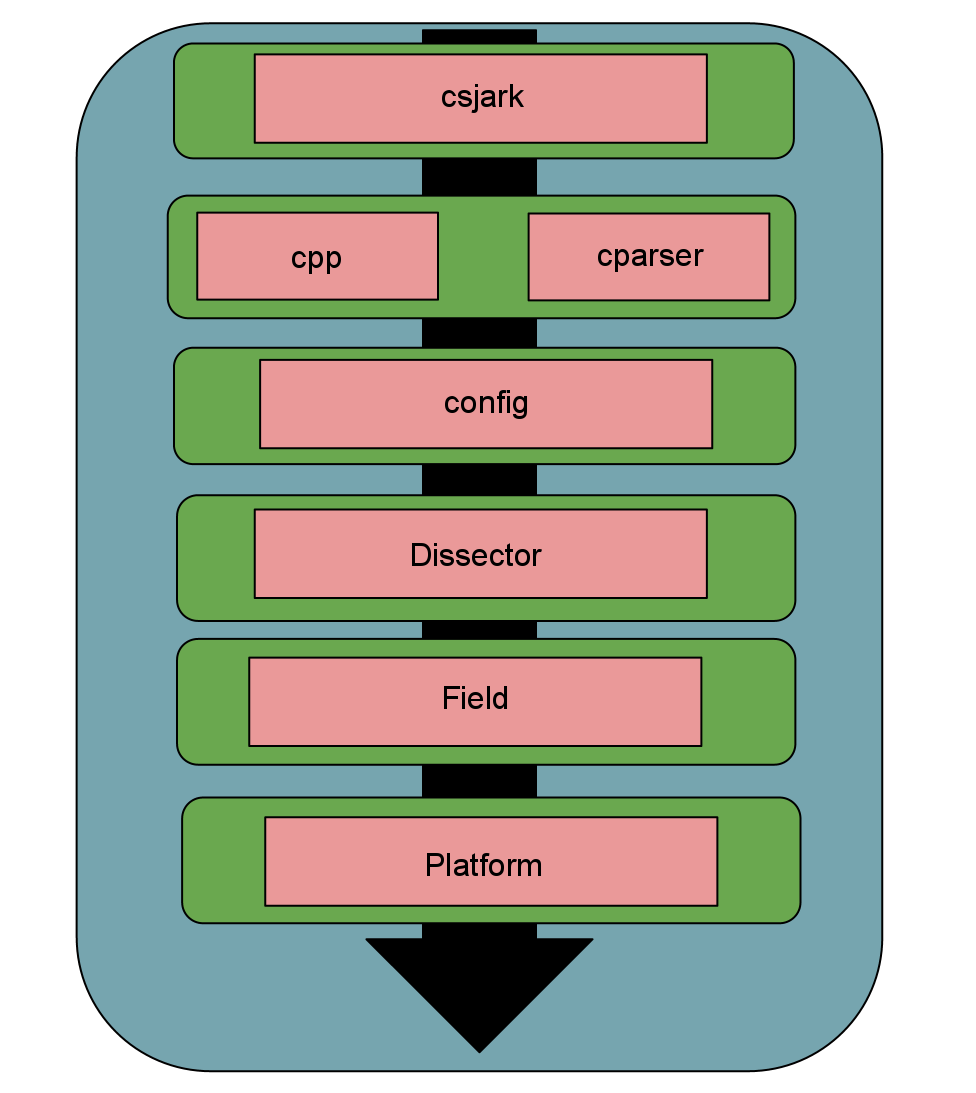
\includegraphics[width=0.7\textwidth]{./planning/img/layered}
	\caption{Layered Architectural Pattern in the \Gls{utility}\label{fig:layered}}
\end{figure}

%----------------------------
\section{Architectural Views}
%----------------------------
This section describes three different views the team used for this project: A logical view, process view and a deployment view.

\subsection{Logical View}
%------------------------
This view shown in \autoref{fig:logicalview}. Command line takes the arguments for \gls{header} file and configuration file as a string. The arguments are parsed in the command line \gls{parser}. Header file is sent to ''\Gls{c} \gls{preprocessor} \& \Gls{c} \gls{parser}'', the \Gls{c} \gls{header} file is loaded and parsed by the \Gls{c} \gls{parser}, whcih generates a parsing tree. Command line also call Configuration, which load the configuration file. The configuration will parse the configuration file and create configuration rules. The \Gls{lua} \gls{script} generator will generate a \Gls{lua} \gls{script} from the parsing tree and the config rules.

\begin{figure}[htb]
	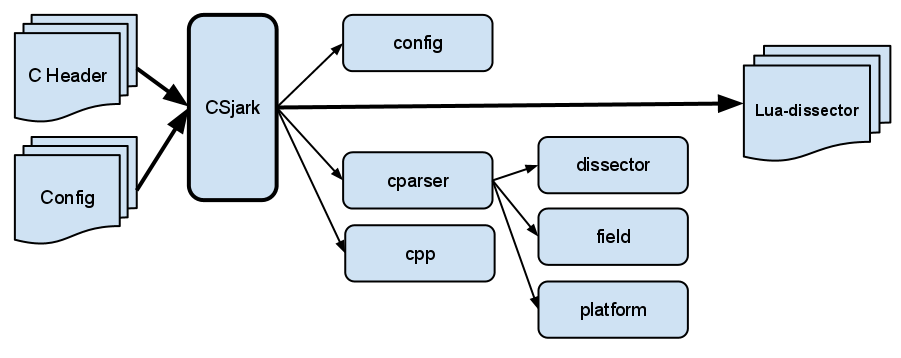
\includegraphics[width=\textwidth]{./planning/img/final_arch}
	\caption{Overall Architecture\label{fig:logicalview}}
\end{figure}

%---------------------
\subsection{Process View}
%---------------------
\autoref{fig:processview} shows the process view for our \gls{utility}. Csjark takes \gls{header} and config files as input and then uses the config and cparser to parse the files. CSjark then uses the cparser to find the \glspl{struct} in the \gls{header} file and then creates \glspl{dissector} for them. These \glspl{dissector} are then written to a file and CSjark then reports to the user by sending a message to the command line.


\begin{figure}[htb]
	\center
	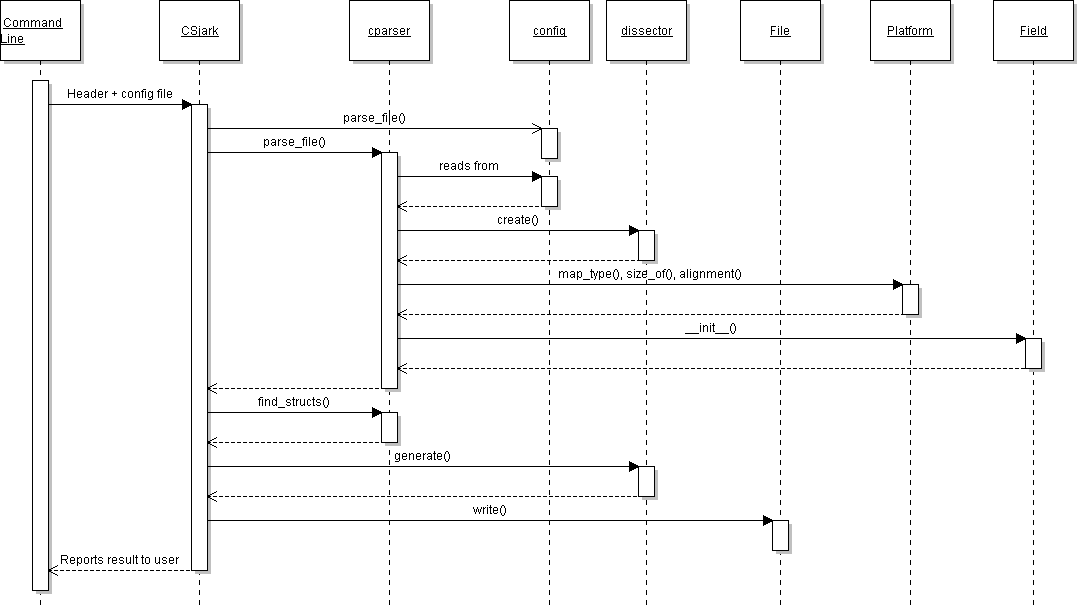
\includegraphics[width = \textwidth]{./evaluation/img/FinalSequenceDiagram}
	\caption{Data Flow During Regular Execution\label{fig:processview}}
\end{figure}


%------------------------
\subsection{Deployment View}
%------------------------

\autoref{fig:deployment} shows the deployment diagram for this project. CSjark 
takes \gls{header}-files and config-files as input, and generates \Gls{lua} 
\glspl{dissector}. All these \glspl{dissector} are added as plugins to 
\Gls{wireshark}, extending the functionality. \Gls{wireshark} will capture the 
data packet when Process A send data to Process B, the \Gls{lua} 
\glspl{dissector} is used to display these data packets correctly.

\begin{figure}[htb]
	\center
	\includegraphics[width = 0.8\textwidth]{./planning/img/Deployment}
	\caption{Deployment View\label{fig:deployment}}
\end{figure}

%--------------------------------
\section{Architectural Rationale}
%--------------------------------
The team decided to use the pipe and filter pattern as the architects felt that it was one of the only architectural patterns that would benefit the \gls{utility} without having to make it needlessly complex. The \gls{utility} was supposed to take \gls{header} files as input and then process the data from them several times, until the end result was a list of \glspl{struct} and \glspl{member} that could be used to make \glspl{dissector} for \Gls{wireshark}. This seemed like an excellent application to use the pipe and filter pattern with, as it would then be easy to add new filters to the \gls{header} file for future increments of the development cycle without having to rewrite what had already been implemented in previous sprints.

The team also decided to use the layered architectural pattern as the code of the utility would have to stay logical and well structured through the entire project if we wanted the future development of the utility to go more smoothly. By dividing the entire utility into several modules and designate layers between them it became easier to decide which functionality would go where in the code which could save the different developers some grief. It would also make the code easier to inspect by whomever that wishes to understand the code and more specifically how the utility works.

For the views the team decided to use a logical view, process view and deployment view. These views were chosen because the architects of the \gls{utility} felt that these views alone could represent the system sufficiently without creating too much overhead for the readers of the document. The logical view supplies the reader with a more in depth view of what the system is comprised of, which is useful for developers who need to figure out the workings of the system. The process view also seemed important for the developers and the testers of the \gls{utility}, as it provides the reader with a more proper overview of the data flow in the system. This makes it a lot easier to see which modules are run when, and to see which external calls dictate the modules' behaviour. Lastly a deployment view was chosen to make it more clear for the reader of the document what the \gls{utility} really produces as output and what other external applications it has to cooperate with. 


%===================
\chapter{Conclusion}
%===================
\label{cha:conclusion}
This chapter describes the final state of the product. It also contains
suggestions on how to improve the utility, as well as a short discussion
on testing, and how it affected our utility.


%------------------------
\section{System Overview}
%------------------------
\autoref{fig:conc:sysow} shows an overview of the final version of the
product. Our utility consist of seven Python modules:
\begin{itemize}
	\item csjark
	\item cpp
	\item cparser
	\item field
	\item dissector
	\item platform
\end{itemize}
The csjark module takes as input C header files and config files. Config
files are forwarded to the config module, which reads them to find rules and
options. The csjark module outputs Lua dissector files.

\begin{figure}[htb]
	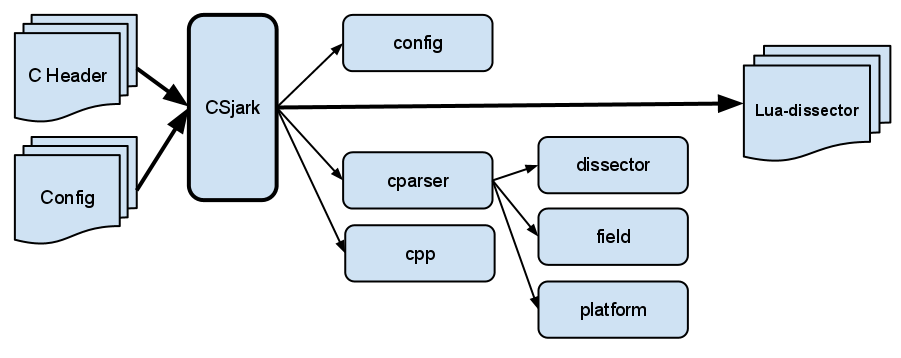
\includegraphics[width=\textwidth]{./planning/img/final_arch}
	\caption{Overall Architecture\label{fig:conc:sysow}}
\end{figure}

Csjark then forwards header files to the cpp module, which calls an external
program, a C preprocessor. The output of the C preprocessor is given to the
cparser module, which forwards it to the pycparser library. An abstract
syntax tree is returned by pycparser, which is traversed by the cparser
module when it searches for struct definitions.

The cparser module creates a Protocol instance from the dissector module for
each struct it finds. The Protocol instance is populated with Field instances
or subclass instances for each struct member.

After all headers have been parsed, the csjark module takes the list of all
protocols created by the cparser module, and writes to file the output of the
generate() function. In the end, it writes the output of the generate function
on a Delegator instance.

The platform module contains platform-specific details, which are used by the
cparser when it creates new fields.

\subsection{System summary}
%--------------------------
Originally, we had some design goals for the product. We wished to have some
logical groupings of functionality into a front-end and back-end. We believe
that we have achieved this goal. Everything specific for generating Lua
dissectors are contained to the field and dissector modules, which contains
no C specific code. These consist of smart data structures which are created
by the front-end, the cpp and cparser module.


%----------------------------
\section{Further Development}
%----------------------------
\label{sec:eval:furtherdev}
This section describes possible improvements to our utility.
In \autoref{sec:conc:optional} we describe how one might implement the remaining
optional requirements, while \autoref{sec:conc:addimps} list other improvements.

\subsection{Optional Requirements}
%---------------------------------
\label{sec:conc:optional}
During the third sprint, as we had completed most of the requirements given to
us, it became clear we would not have sufficient requirements for a fourth
sprint. We requested more possible features from the customer, who provided us
with a list of new functional requirements and their prioritization.

In the fourth sprint planning meeting, we estimated the work hours needed to
complete each of the new requirements, including implementation, testing and
documentation. Based on the customers prioritization and our estimates, we
classified four of them as optional, as we did not deem it possible to
fulfill them in the fourth sprint.

The customer asked us to provide a description of how the unfulfilled
requirements could be implemented, which is listed below.
\begin{enumerate}
\item Don't regenerate dissectors across multiple runs
\item Use Doxygen comments for "Description"	
\item Read int-enum config from header files
\item Display if struct member contains uninitialized memory
\end{enumerate}

\noindent The following paragraphs describe how they can be implemented.
\paragraph{Don't regenerate dissectors across multiple runs}
To be able to decide if we have already generated dissectors in earlier runs, we need to store some state on disk. 

We need to store the last modified timestamp, which the operating system reports, at the time we last read them. 
This needs to be done for each single input file, both header- and config files.
Since command line arguments will affect the output, they must also be stored. The main challenge with this task is the fact that handling \#include directives are performed by the external C preprocessor program, so we will not know which files need to be considered when evaluating, if files have been modified since last run.

One could look at \#line directives outputted by the C preprocessor before we start parsing files, but the benefit of not regenerating dissectors would be diminished.

We estimate this task would require implementing our own C preprocessor or using a library instead of an external tool, to be able to extract the needed file dependencies. Our utility depends on PLY, which have a 95\% finished implementation of a C preprocessor, which might prove valuable for this task.

When we are able to know which files depend on each other, and the last time they were modified, the task is simply to find a suitable data structure to store on disk between runs.

\paragraph{Use Doxygen comments for "Description"}
Comments are removed by the C preprocessor, which means we must parse them before it is run. As the preprocessor evaluates which files to open, we would be required to implement our own or use a library, or try to evaluate applicable files in all include folders.

The task, if such support was available, would simply be to search for doxygen comments, and when one is found parse it to extract the correct information.

\paragraph{Read int-enum config from header files}
Integers, which should act as enums in Wireshark, are defined by some specific C preprocessor macro define directives in the customer's current header files. This task is to automatically extract such information, to require less manual configuration of our utility.

Like the two previous task, this will require us to parse C preprocessor directives before they are removed by the C preprocessor, which means we must implement our own C preprocessor or use a library.

To avoid having to parse both C preprocessor directives and C code at the same time, we could design a syntax for describing which struct member(s) the macro define directives refer to. For example \#define BEGIN\_CSJARK\_ENUM\_FOR\_NAME could be placed right before the current enum macro directives start, which would tell us that they refer to struct member NAME.

This task becomes trivial to implement if we had a custom C preprocessor we could modify.

\paragraph{Display if struct member contains uninitialized memory}
Uninitialized memory will look different depending on the compiler, so therefore we need to add support for specifying how it will look for each Platform instance in platform module. Since we can only evaluate the actual memory on the Wireshark end of things, most of the functionality must be written in Lua code.

These two conditions suggest that the dissector module should, inside the Delegator class, generate a suitable Lua function in luastructs.lua which accepts a buffer value for a field and the field node. This function should, if the buffer value match uninitialized memory, set an appropriate warning on the field node.

This new function must be called for every field defined in every dissector we generate, inside the appropriate dissector functions.

In addition to implementation, the task involves researching how uninitialized memory looks on different platforms we support, and creating pcap files for testing the functionality.

\subsection{Additional Improvements}
%-----------------------------------
\label{sec:conc:addimps}
In \autoref{sec:sp4:onsite} we described testing of our utility on customer's
code base. We discovered several corner cases which we did not support, and we
also found problems with memory consumption when number of input files was
over 1000. These problems could be solved by further development, which we
describe in following paragraphs.

\paragraph{Reduce memory consumption}
We did some basic profiling, both of memory and CPU usage, to evaluate what
could be improved. Almost all CPU usage was defined to the preprocessor and
the pycparser library, which means we could not find any possible improvements
in out utility.

Memory profiling on 1000 header files revealed that almost all memory was used
by Python dictionaries and lists. Our utility builds up a list of Protocol
instances which represent all structs we parse, before we write any to disk.
This grows as more files are parsed. A simple, but effective, solution would
be to write Protocols to disk as after we have parsed a single file. We would
still need to store a few attributes for each Protocol, such as name, id,
size. We believe this would reduce memory consumption sufficiently.

It is also possible that we leak some memory each time we fail to parse a
file, which could be investigated and fixed afterwards.

\paragraph{Additional C parsing support}
We successfully parsed 160 of 200 header files in customer's include folder,
the remaining files failed mostly from corner cases our utility did not
support, for example typedef's we had not considered. We believe it would be
relatively easy to add further support for them when they are discovered.

\paragraph{Less manual configuration}
Several of the optional requirements are focused on requiring less manual
configuration. If we perform the C preprocessing ourself instead of delegating
it to an external program, we would be able to read configuration from
comments and \#define's inside the header files.

%----------------
\section{Testing}
%----------------
At the beginning of the project all of the team members agreed that we were going to focus on doing extensive and proper testing of our utility. In this section we will discuss whether or not we were able to reach the goals we sat at the beginning and during the project.

\subsection{Methods}
%-------------------
At the beginning of the project we only used black box test cases and unit tests. We quickly found that even though we were able to uncover several bugs using these methods, it was hard to calculate what and how many parts of the system were actually undergoing testing. This again made it difficult to figure out the real quality of our tests and if our testing efforts were used to their true potential. When we then decided to use a tool for calculating code coverage, we noticed that there were large parts of the system that were still untested, even though the functionality of the system had been tested in our black box test cases. We therefore made a goal of trying to have a test coverage of at least 80\% in order to catch as many bugs as possible. This proved to be a hard task at first, but as can be seen in \autoref{fig:sp4CoverageChart}, once we got used to using a tool to calculate the coverage of our unit tests, we were able to improve the quality of our tests so that they covered more parts of the system.

\begin{figure}[htb]
	\center
	
\includegraphics[width=\textwidth]{./sprints/img/sprint4_code_coverage_chart}
	\caption{Code Coverage Progress from Previous Sprints\label{fig:sp4CoverageChart}}
\end{figure}

\subsection{Testing Conclusion}
%------------------------------
After finishing the project we had uncovered several serious and many more non-critical bugs in our utility. We also discovered several bugs in the Lua-implementation of Wireshark that we needed to have our customer to fix. This proved to be very important as this severely reduced the amounts of bug fixes that had to be implemented, after being allowed to send our developers to work with the utility at the customer-site. We were therefore able to create a working product within the small time-frame we had left after testing the utility at the customer-site. We therefore conclude that it had indeed been necessary to focus on creating extensive tests for the utility and that the methods we had chosen for testing were sufficient to get a working end-product.


%----------------
\section{Summary}
%----------------
The team was given the task of creating an utility for automatic generation of dissectors for C structs in Wireshark. The dissectors were supposed to be created for structs contained in the customer's C header files so that they could be used to decode their \gls{ipc}.

After finishing the product, the customer reviewed the utility and they were satisfied with what we had delivered. We also managed to complete all of the initial functional requirements, all of the non-functional requirements and all other functional requirements that were not considered optional. The team firmly believes that the customer will be able to use the utility for its intended purpose, without having to do much additional work. This makes it feasible for them to use Wireshark for debugging inter-process communication. We therefore feel that we have delivered a solution to the task that the customer presented to us in the beginning of the project.


%===========================
\chapter{Project Evaluation}
%===========================
This chapter gives an evaluation of the project and the course, TDT4290 Customer Driven Project. The main focus is to describe the how the team evolved and how work was done during the project.   

%----------------------------------
\section{Team Dynamics}
%----------------------------------
The forming and development of the team are described in this section.
%----------------------------------
\subsection{Goals and Team Building}
%----------------------------------
The project started out with randomly assigned student groups of six to seven people. This was done intentionally to learn the students to work in a realistic setting. Our group consisted of six Norwegian students and one Czech student. 

As one of the team members was a foreign student, all the internal team communication had to be done in english. In addition our advisors were english speaking, so the whole project was done in english. This did not occur as a problem, because all the team members both spoke and wrote english fluently.

At the first meeting we decided to state our personal goals for the project. This resulted in the following list:
\begin{itemize}
	\item Improve programming skills.
	\item Learn to develop software efficiently.
	\item Learn to work in a realistic environment.
	\item Fulfill the needs of the customer. 
\end{itemize}
These goals match the course's goals, with some extensions. All these goals was common for the team members, which resulted in good cooperation from the start and an agreement of what we wanted to achieve in the project. The decision to characterize ourselves as a team came early in the project, which is defined to be a collection of people working interdependently and is committed to achieve one common goal.

None of the team members had any relations with each other when the project started. During the project we learned how to work together in a professionally and efficient manner. Getting there was a demanding task and is described more thoroughly in the section regarding team evolution.

\subsection{Team Evolution}
%---------------------------------
During the first weeks of the project the team were in a good, but also uncertain stage. The team members did not know the boundaries of the others and tried to not end up in an argument. This resulted in a series of matters; responsibility for tasks were not taken and no one dared to ask why tasks was not done.

The team realized the problems.

\section{Risk Handling}
%----------------------------------
Some of the risks predicted in the planning phase occured to a certain degree during the project.
This section will discuss those risks and how they were handled.

\paragraph{R4. Illness/Absence}
In general, not many team members were absent for longer periods.
One team member was away in northern Norway for a week on vacation, and another was sick for a week and a half. This caused some delay on a few tasks, as the absentees had to get up to date on the state of the project, but it did not majorly hinder the progress of the team. The consequence of this risk was also diminished by the fact that it occured early in the project, and that the team members who were absent did not work on critical tasks at the time.

\paragraph{R6. Conflicts within team}
In the start of the project, the team members were divided on which tools to use, and on which programming language to use. Because of this, the team had to spend some time discussing back and forth. After some constructive discussions the team was able to come to a mutual decision.

Also, some team members felt that it was not realistic that the course should demand 25 hours from each member. As the project progressed, it quickly became apparent that this number of hours were needed to complete the project in a satisfying manner. This led to an overall increase in work effort in the team.

\paragraph{R8. Miscommunication within team}
During sprint 3, the ones responsible for creating test data and the ones writing the test cases did not clearly communicate with each other. This led to having to make small changes in some of the test cases to be able to use the test data.

The test responsible wrote test cases for functionality that the programming team had not thought about. For example, checking that you are not allowed two platforms with the same platform ID.
When the problem was detected, all essential functionality was added.

\paragraph{R10. Lack of experience with Scrum}
As the team had no previous experience with Scrum, the project got off to a slow start.
After evaluating the first sprint, it quickly became apparent that the process was far from perfect.
The second sprint was an improvement of the first, and the planning meeting was longer and more detailed, but in our opinion it was still not good enough. We felt that we did not adhere to proper Scrum, and that we did not properly explain the different tasks in the backlog. In the last two sprints, we felt that we had achieved a better understanding, and this really showed in the process. A more detailed discussion can be found in the Scrum section.

\paragraph{R11. Requirements added or modified late in the project}
At the customer meeting on the first day of sprint 4, the customer suggested several new requirements that they would like is to implement. Some requirements were also modified, as we had not implemented them exactly the way they wanted us to.

As we had to focus on tweaking some functionalities to work on their code, and also had to spend time on writing the report, we had to tell the customer that we would probably not be able to finish all the new requirements. This is because implementing a requirement would also require testing, user documentation and additional report work, which is something we could not afford to allot time for.


%--------------------------------
\section{The Process}
%under construction!
%--------------------------------
TODO: Sondre

%-----------------
\subsection{Scrum}
%-----------------
During the preliminary study, we decided to use an agile development method, 
to be able to adopt to changes in requirement during the project, so we 
decided to use Scrum. None of the team member had any previous experience with 
Scrum. In the beginning of the course we had a lecture about Scrum, and we 
got a basic insight in how Scrum works.

When the first sprint planning was finished, we understood that we did not 
follow Scrum properly. The meeting was very short, and we did not do any 
design during the sprint planning. The work items from the sprint was wrong 
estimated, and was not divided propely into work items. For each sprints we 
improved, and the scrum process was good in the end of the project.

Some of team members feel that we followed Scrum to strict, instead of doing 
what that was best for the project. In the end of the project we needed to use 
much time on fixing the utility so it run on the customer's code, since we 
could not change our sprint plan, we ended up with a very high workload.

During the project we learned the advantages of using Scrum, since we could 
get some feedback on the work we had done from the customer, and then improve 
the features to what the customer exactly wanted. 

%------------------------
\section{Time Estimation}
%------------------------
In total there was estimated a total of 2275 hours for this project. We put a 
little more effort in this project and ended up on 2331 hours. This mean we 
was a little over the estimate, and the reason mainly because we wanted to the 
utility work for the customer and a decent amount of work on the report in the 
end of the project. 

The work breakdown structures in \autoref{tab:wbs}, shows the estimated and 
actual hours for each task. The estimates are quite good on most of the task, 
for project management we have used 454 hours, and 275 hours was estimated. 
The reason that we used so many houes on project management is that we had 
weekly meeting with both customer and advisor. In addition to this we had 
internal meetings in the team, and all daily Scrum meeting was registered as 
Project Management. In the start of the project some of the effort was 
registered, so the amount of time spent on project managemnt is actual lower.

In each of the sprints we estimated time for the work items. The estimation 
was based on that every team member should be able to finish the task on the 
estimated time. So in total the work items was overestimated, because some 
team members had more experience, and could finish the task much faster.

The time distribution by task is shown in \autoref{fig:time_by_task}. Nearly 
20\% of the time was used on the project management, for the planning, 
preliminary studies and requirement specificaiton was approximate 10\%, 
actually is this higher, because of some wrong registration of effort in the 
start of the project. The total time that was used for the sprints was over 
40\%., which is a good amount for the development of CSjark. 

\begin{figure}[htb]
	\center
	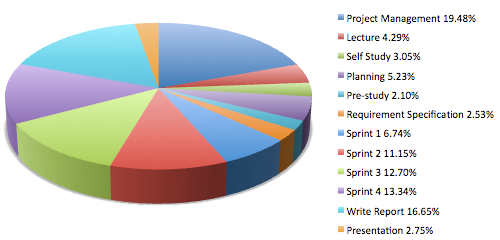
\includegraphics[width=\textwidth]{./evaluation/img/piechart_time}
	\caption{Time Distribution by Task\label{fig:time_by_task}}
\end{figure}

In the start of the project there was low activity, but effort per week 
increased during the project. Effort registered per week can be seen in 
\autoref{fig:time_by_week}. To achieve the 2275 hours in total for the 
project, 175 hours per week was needed. The effort in week 12 was high because 
we needed to finish the last sprint and very much work on the report was done.

\begin{figure}[htb]
	\center
	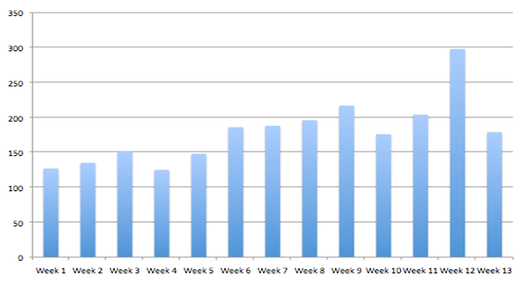
\includegraphics[width=\textwidth]{./evaluation/img/columnchart_effort} 
	\caption{Time Distribution by Week\label{fig:time_by_week}}
\end{figure}

%-------------------------------
\section{Quality Assurance}
%-------------------------------
At the start of the project we made several plans for ensuring quality of the project. This section discusses which of those plans did not work out and what we ended up doing instead.

Initially we planned that we would have peer review of all of the code written for the utility. This plan was something that we were unable to follow up on, mostly due to the poor planning meetings in sprint one and two where the time needed for pair review was not taken into consideration. This made it difficult to organize who was going to do the peer reviews and how we were supposed to find the time to do them. In the end, the lead programmer ended up reviewing most of the code written by the other developers, but the group consensus was that the quality of the code was good enough that it would have been irresponsible to spend more time on peer reviews.

During every sprint the team was supposed to provide the advisor with up to date information regarding the report and the progress with the utility. This was not followed up on as the team members did not want to submit unfinished work to the advisor. This proved to be a problem towards the end of the project forcing the team to start submitting more of the report work to the advisor. As this was not done earlier in the project, the team instead had to organize for several of the members to go through the early stages of the report and raise the quality of the documents internally.

It was planned that the team member responsible for the document was supposed to keep a bird's eye view of the report and go through the different entries before the end of each sprint. This proved to be too much work for just one person. We therefore also made sure that in several other team members would support the one responsible for having a proper overview of the report 

%----------------
\section{Learning Process}
%----------------
TODO: Sondre

%----------------
\section{Customer Relations}
%----------------
Our relationship with the customer was good throughout the entire project.
We were assigned two customer representatives. As they were developers themselves, they both had a technical background. This made it easier to communicate with the customer.
They knew exactly what they wanted, and were more than happy to give feedback and tips on the implementation of the different requirements. When we first received the initial requirements, we did not fully understand them. After some meetings and dicussions, both internally and with the customer, the team was able to provide the customer with a clear requirement specification that they accepted.

One of the customer contacts was a member of Wireshark's core development team. When we discovered bugs in Wireshark, he could fix them and apply a patch. He also had insight into how 
Lua dissectors were built, and how they interacted with Wireshark. This was a major asset to the team. When we encountered problems during implementation, the customer was able to give us invaluable feedback on how to proceed. This is something that a less technical customer would not have been able to give us.

Each week we had a meeting with the customer where we demonstrated the requirements we had implemented since last meeting. The customer then gave us feedback on the functionalities, and told us what we had to change or improve. This way, any misunderstandings were detected and dealt with in a swift manner.

The customer contacts also had access to our repository, thus they could test the utility themselves.
This meant that they could get a first hand-experience of the utility, and could more easily detect bugs and other issues.	

A problem we had was that, due to security issues, Thales could not allow us to test our utility on their source code. This meant that we had to do some guessing during the implementation, and getting the utility to work on their code was a difficult process. Luckily, Thales gave us the opportunity to send two of our members to them for a few days, as documented in the test section of sprint 4. That gave us an opportunity to fix most of the bugs that we encountered, and in the end the customer said that they were happy with our utility. They approved all the requirements we had listed, although a few of the optional requirements were not implemented due to time constraints.
Overall the customer felt that we were flexible, and adhered to most of their needs.

The week before the end of the project, the team had a presentation at Thales for our advisor, the customer contacts, and some other employees of Thales. The employees that were there are probable users of the dissectors that our utility creates. Due to this, the presentation was focused on the demonstration of the utility, where we showed how the structs were dissected in Wireshark.

The customer also got one of their co-workers to read CSjark's user manual.
The user manual was a little too unclear in some parts, so we used that feedback to improve it, and increase its quality.

The team felt that we were lucky with the customer that we were assigned.
The fact that they knew exactly what they wanted, had a technical background and showed great enthusiasm for the project, made the project more manageable. This also increased the motivation for the team. We felt that they were interested in what we were developing, which ensured a good meeting atmosphere and a good working relationship. Throughout the entire project, they gave us essential feedback on the implementation and requirements, and they were not afraid to tell us if we did something that they disagreed with. The fact that we had two customer contacts, instead of one, increased the amount of feedback we received, and also meant that there was always one person available for us to contact. All in all, we could not be more satisfied with our customer.


%----------------
\section{Summary}
%----------------


\end{document}

